\documentclass{beamer}
\bibliographystyle{amsalpha}
\usepackage{cite}
\usepackage[normalem]{ulem}
\setbeamertemplate{footline}[frame number]{}
\setbeamertemplate{navigation symbols}{}

\title{The Heterogeneous Multiscale Method for Plasma Modeling}
\author[Price and Shohet]{Jake Price and Gil Shohet}
\institute[CPSSW]{Computational Physics Student Summer Workshop}
\date{\today}

\begin{document}
\begin{frame}
\titlepage
\end{frame}

\begin{frame}
\frametitle{What is multiscale?}
\begin{columns}[T] 
\begin{column}{.48\textwidth}
\vspace{0.9cm}
``[Multiscale methods] include analytical and numerical techniques that exploit the disparity of scales, as well as multi-physics problems...What we have in mind are problems that involve physical laws at different levels of detail, such as quantum mechanics and continuum models.''\\
\hfill
\\\hfill-Weinan E
\end{column}%

\hfill%

\begin{column}{.48\textwidth}
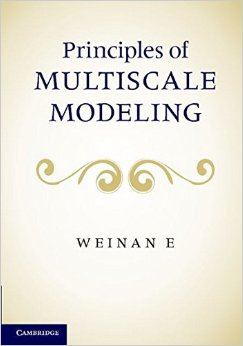
\includegraphics[width=\textwidth]{principles.jpg}
\end{column}%
\end{columns}
\end{frame}

\begin{frame}
\frametitle{What is heterogeneous multiscale method?}
``HMM is a framework for linking models at different scales. It follows a top-down strategy: The basic starting point is an incomplete macroscale model, with the microscale model used as a supplement. It consists of two main components: The macroscale solver and a procedure for estimating the missing numerical data from the microscale model."\\\hfill\\\hfill -Weinan E, et. al.
\end{frame}

\begin{frame}
\frametitle{Our goal}
\begin{itemize}

\item Establish a computational framework for multiscale plasma modeling as a proof of concept
\vspace{1em}
\item Macroscopic model: Kinetic theory using the BGK approximation of the Boltzmann equation (BGK)
\vspace{1em}
\item Microscopic model: Molecular dynamics (MD)



\end{itemize}
\end{frame}


\begin{frame}
\frametitle{Problem statement}
\begin{itemize}
\item Ionized particles confined to a small two-dimensional periodic domain that varies in the $x$ direction and is uniformly distributed in the $y$ direction\vspace{1em}
\begin{itemize}
\item May have multiple species with different masses and charges\vspace{1em}
\end{itemize}\item Experimental setups for studying ``dusty plasma'' often utilize a similar domain\vspace{1em}
\item The framework is general, and could be extended to more dimensions with different boundary conditions
\end{itemize}
\end{frame}

\begin{frame}
\frametitle{Macroscale model}
The 1D-2V BGK approximation of the Boltzmann equation is:
\[\frac{\partial f}{\partial t}+v_x\frac{\partial f}{\partial x}-\frac{Z}{m}E(x)\frac{\partial f}{\partial v_x}=\frac{f_{eq}-f}{\tau}
\]\begin{itemize}
\item $f(x,v,t)$ is the distribution function for the species\vspace{0.5em}
\begin{itemize}
\item If there are multiple species, there is an $f_i(x,v,t)$ for each with associated $m_i$, $Z_i$, $\tau_i$, and $f_{eq}^{(i)}$\vspace{0.5em}
\item Assumed to be uniform in the $y$ direction\vspace{1em}
\end{itemize}
\item $v_x\frac{\partial f}{\partial x}$ is an advection term\vspace{0.5em}
\item $-\frac{Z}{m}E(x)\frac{\partial f}{\partial v_x}$ is a response to the electric field\vspace{0.5em}
\item $\frac{f_{eq}-f}{\tau}$ relaxes the solution toward an equilibrium distribution $f_{eq}$ with relaxation time $\tau$
\end{itemize}
\end{frame}

\begin{frame}
\frametitle{Macroscale model comments}
\begin{itemize}
\item The $E(x)$ term is found by solving the nonlinear Poisson equation
\[-\frac{\epsilon_0}{4\pi}\phi_{xx}=\sum_iZ_in_i(x)-en_ee^{\frac{e}{T_e}\phi}
\]and using $E(x)=\phi_x$\vspace{1em}

\end{itemize}
\end{frame}


\begin{frame}
\frametitle{Microscale model}
\begin{itemize}
\item The microscale model is two-dimensional in space and velocity\vspace{0.5em}
\item Individual ions exert forces through the electric potential
\[V_{ij}=\frac{z_iz_j}{r_{ij}}e^{-\frac{r_{ij}}{\lambda_{de}}}
\]where $\lambda_{de}$ is the Debye length representing charge screening by the background electrons \vspace{0.5em}
\item The force is given by
\[f_{ij}=V_{ij}\left(\frac{1}{r_{ij}}+\frac{1}{\lambda_{de}}\right)
\]
\item The governing equation for each particle is the ODE
\[\dot{x}=v,\;\;\dot{v}=\frac{f}{m}
\]
\end{itemize}
\end{frame}

\begin{frame}
\frametitle{Connecting the macroscale to the microscale}
``These are problems for which a closed macroscopic model should exist for a properly selected set of macroscopic variables, but the macroscale model is not explicit enough to be used directly as an efficient computational tool.''\\\hfill Weinan E, et. al.
\vspace{1em}
\begin{itemize}
\item The missing ingredient is the timescale $\tau$ of relaxation to equilibrium\vspace{1em}

\end{itemize}
\end{frame}


\begin{frame}
\frametitle{Connecting the macroscale to the microscale}
\begin{itemize}
\item We can simulate the molecular dynamics in full detail, but it is much more computationally expensive than the BGK simulation\end{itemize}



\begin{itemize}
\item Idea: Use short MD simulations to approximate $\tau$ for use in BGK simulations on a macroscopic timescale
\end{itemize}
\begin{center}
\includegraphics[width=0.3\textwidth]{lightbulb.jpg}\end{center}
\end{frame}

\begin{frame}
\frametitle{Challenges}
\begin{itemize}
\item As the BGK simulation runs, the relaxation time $\tau$ becomes ``stale''\vspace{1em}
\begin{itemize}
\item $\tau$ reflects the relaxation time of the initial distribution as simulated in the MD precomputing step\vspace{1em}
\item As the distribution changes considerably, the relaxation timescale changes as well\vspace{1em}
\end{itemize}
\item Solution: Periodically return to the microscale, simulate for brief time, and update $\tau$
\end{itemize}
\end{frame}

\begin{frame}
\frametitle{Challenges}
\hspace*{3.5em}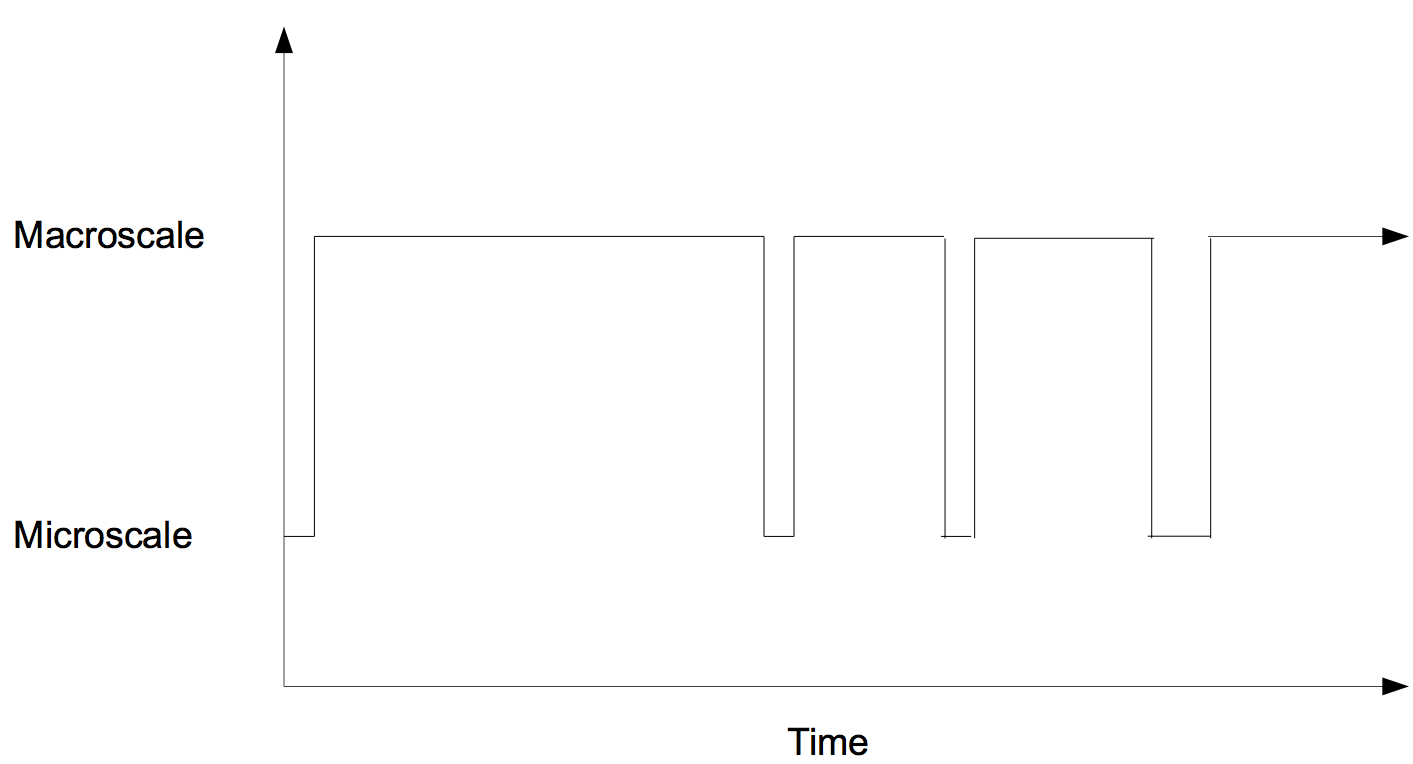
\includegraphics[width=0.65\textwidth]{scheme.png}
\begin{itemize}
\item How to compute $\tau$ from the microscale simulation?
\item How long to run the microscale simulation for reliable $\tau$?
\item How long to run macroscale simulation before returning to update $\tau$?
\item How to downsample the macroscale distribution for a microscale initial condition?
\end{itemize}
\end{frame}

\begin{frame}[t]
\frametitle{Challenges}
\tiny \begin{itemize}
\item[\tiny$\bullet$] How to compute $\tau$ from the microscale simulation?
\item[\tiny$\bullet$] How long to run the microscale simulation for reliable $\tau$?
\item[\tiny$\bullet$] How long to run macroscale simulation before returning to update $\tau$
\item[\tiny$\bullet$] How to sample the macroscale distribution for a microscale initial condition?
\end{itemize}\vspace{6em}
\normalsize
\begin{itemize}
\item The relaxation time computation might be computed by tracking the rates of change of the moments of the MD distribution
\vspace{1em}
\item The second two challenges will require experimentation
\end{itemize}
\end{frame}

\begin{frame}[t]
\frametitle{Challenges}
\tiny \begin{itemize}
\item[\tiny$\bullet$] \sout{How to compute $\tau$ from the microscale simulation?}
\item[\tiny$\bullet$] \sout{How long to run the microscale simulation for reliable $\tau$?}
\item[\tiny$\bullet$] \sout{How long to run macroscale simulation before returning to update $\tau$?}
\item[\tiny$\bullet$] How to sample the macroscale distribution for a microscale initial condition?
\end{itemize}\vspace{1em}
\normalsize
\begin{itemize}
\item Of these challenges, the most difficult one is sampling the macroscale distribution to get a consistent microscale state\vspace{0.5em}
\begin{itemize}
\item If we sample naively, particles that are placed very close to one another could lead to a sharp total energy increase\vspace{0.5em}
\item It is easy to maintain consistent density and velocity distributions between scales, but not temperature\vspace{0.5em}
\end{itemize}
\item Possible solution: Use a thermostat to drive an initial guess at the distribution to the proper temperature, tweak positions and velocities from here to achieve consistent densities and velocities
\end{itemize}
\end{frame}





\begin{frame}
\frametitle{Where we are now}
\begin{itemize}
\item At present, we have working code for simulating MD with two spatial and two velocity dimensions, as well as for simulating BGK with one spatial and two velocity dimensions
\vspace{1em}
\begin{itemize}\item Both can take a variety of initial conditions, including $n$ species with different masses and charges (i.e. for a mixing problem)\vspace{1em}
\end{itemize}

\item The code is being tested for bugs, and we will soon begin linking the two
\vspace{1em}
\item Our goal is to choose a regime in which the MD simulation can be computed in full over a long time period, and compare this against a (much faster) multiscale scheme
\end{itemize}\vspace{1em}\begin{center}\large \textbf{Demo!}\end{center}
\end{frame}

\begin{frame}
\begin{center}\huge Questions?\end{center}
\end{frame}


\end{document}